\section{MVC - \emph{Model View Controller.}}
\begin{frame}{Titulo}
\begin{block}{}
	\begin{itemize}
		\item Patr\'on de diseño que separa al modelo de datos, la lógica de control de la aplicaci\'on y la interfaz de usuario en tres componentes distintos.
	\end{itemize}
\end{block}
\end{frame}


%\begin{frame}{Tips - Ocultamiento de Informaci\'on - Ejemplo.}
  %\begin{figure}
    %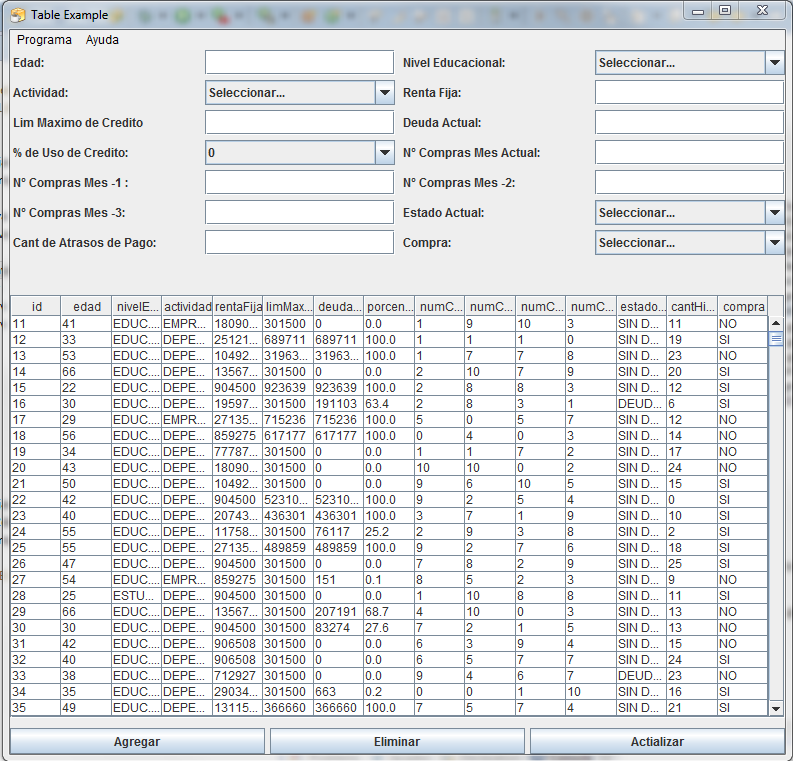
\includegraphics[scale=0.3]{figuras/DT.PNG}
  %\end{figure}
%\end{frame}

%\begin{frame}{Manejo de Excepciones - try, catch, finally}
%\begin{block}{Ejemplo.}
%\lstinputlisting[language=Java,caption={},numbers=none]{resources/excepciones/Finally.java}
%\end{block}
%\end{frame}
